\section{Proposal Discussion}
\label{sec:sec007}

Through iterative development with four clinicians, we consolidated the following fundamental features to cover an assertiveness-based interaction.
In our prior work (Figure~\ref{fig:fig002}), we considered a medical image as the main input and attempted to exhaust all possible diagnoses.
However, clinicians often have a specific question for a breast image.
Sometimes, with important contextual information among the several clinical co-variables.
For instance, C11 (Senior) and C15 (Junior) mentioned that ``In breast cancer, some image patterns will result in a more severe prognosis depending if the patient has [co-variables] personal and/or family history''.
Also, C11 suggested that the assistant agent could alert radiologists about this available co-variables, which will substantiate the case severity.

By taking it into account, we can affirm ({\it i.e.}, in an assertive-based strategy) those co-variables.
Therefore, the assistant will justify the diagnostic and advise the clinician to make the right decision.
However, it is important to balance the affirmation levels depending on the group of medical experience.
In fact, during our focus groups (Section~\ref{sec:sec00502}), C11 (Senior) tend to prefer a more {\bf Non-Assertive} communication.
On the contrary, less experienced clinicians, such as C5 (Intern) and C15 (Junior), preferred a more {\bf Assertive} communication.

\subsection{Initial User Interface}
\label{sec:sec00701}

Concerning the assertiveness-based interactions, we will adapt the old version (Figure~\ref{fig:fig002}) of our assistant converging to the new (Figure~\ref{fig:fig024}) one.
For the new version (Figure~\ref{fig:fig024}), we will have two prototypes.
One prototype to simulate the {\bf Assertive} scenario and another to simulate the {\bf Non-Assertive} scenario.

To fulfill this document design goals (Section~\ref{sec:sec00303}), raised from a later study, we will need to keep the following feature characteristics.
First of all, when advising clinicians for the correct use of the various modalities ({\bf MID}), we have to provide the {\it 5.3.~Modality~Selection} feature (Figure~\ref{fig:fig002}) on a {\it Multimodality} perspective.
Second, we must provide clinicians' free choice with both {\it 6.2.~Accept} and {\it 6.3.~Reject} options, so that the clinician can control ({\bf CRD}) the final answer.
Third and final, the assistant agent must substantiate the decision with co-variable explanations ({\bf BED}).

\subsection{Proposed Assistant}
\label{sec:sec00702}

As shown in Figure~\ref{fig:fig026}, the main interface of {\it BreastScreening-AI} (Figure~\ref{fig:fig024}) will embrace two scenarios: (1) {\bf Assertive}; or (2) {\bf Non-Assertive}; and two agent behaviours: (i) {\bf Proactive}; or (ii) {\bf Reactive}.
For Figure~\ref{fig:fig026}.a, the agent presents proactively the set of available co-variables outputted by our AI models and the respective accuracy.
The communication is {\bf Assertive}, meaning that the assistant substantiate the information with affirmative sentences.
Immediately, the clinician can {\bf Accept} or {\bf Reject} the assistant suggestion.
For Figure~\ref{fig:fig026}.b, the agent first present a summary of the suggested result.
After that, for this example, if the clinician press the {\bf Accept} button, it will present ({\it e.g.}, {\bf Reactive}) a more detailed information in a less affirmative ({\it i.e.}, {\bf Non-Assertive}) way.
From there, the clinician can confirm the suggestion or go {\bf Back} to {\bf Reject} the result.
With this strategies, we will try to convince the clinician to provide the best answer.
Therefore, we expect to mitigate the medical error by reducing the rates of FPs and FNs.

\subsection{Contextualizing Impressions}
\label{sec:sec00703}

All four clinicians reacted positively to our initial idea of adapting the agent according to the respective medical experience.
More precisely, C11 (Senior) mentioned during our focus group (Section~\ref{sec:sec00502}) that, the more quick and effective the communication is, the better.
Giving us an idea that Senior clinicians typically prefer ({\bf RQ2.}) a {\bf Non-Assertive} and {\bf Proactive} scenario.
On the contrary, C15 (Junior) argued that giving the last chance ({\it e.g.}, {\bf Reactive}) when validating the assistant classification with affirmative ({\it i.e.}, {\bf Assertive}) substantiation, would be important.

%%%%%%%%%%%%%%%%%%%%%%%%%%%%%%%%%%%%%%%%%%%%%%%%%%%
\begin{figure*}[htbp]
\centering
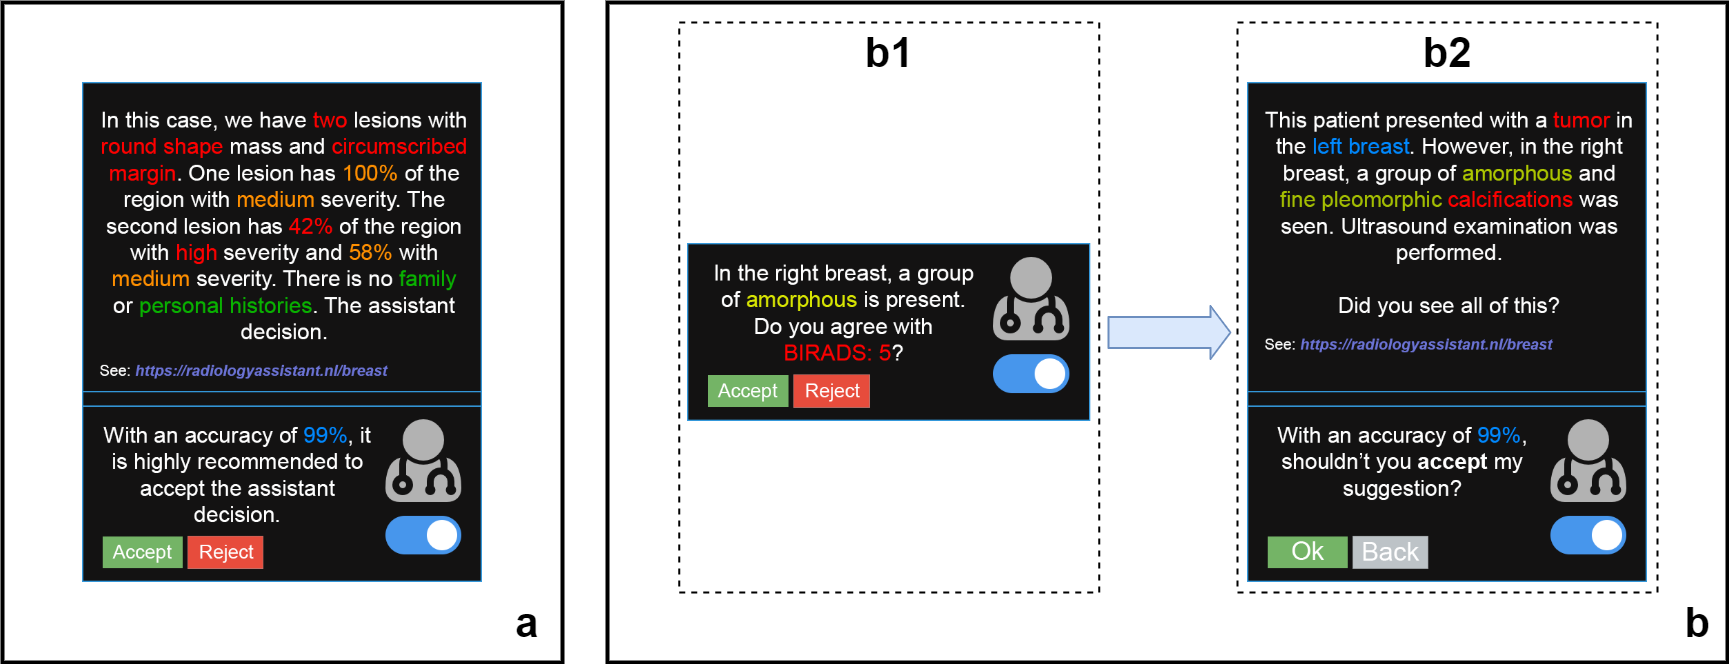
\includegraphics[width=1.00\textwidth]{fig026}
\caption{Assistant agents with several scenarios and behaviours. We have the (a) first scenario, {\it i.e.}, an {\bf Assertive} agent with a {\bf Proactive} behaviour. Next, we have the (b) second scenario, {\it i.e.}, a {\bf Non-Assertive} agent with a {\bf Reactive} behaviour. In the {\bf Non-Assertive} scenario and {\bf Reactive} behaviour, the agent first show the (b1) summarized suggestion and then shows the (b2) detailed information.}
\label{fig:fig026}
\end{figure*}
%%%%%%%%%%%%%%%%%%%%%%%%%%%%%%%%%%%%%%%%%%%%%%%%%%%

\subsection{Comparison Across Clinicians}
\label{sec:sec00704}

In a future study, we will introduce the 2x2 experimental settings that will be used to test the performance ({\bf RQ1.}), perception ({\bf RQ2.}) and UX ({\bf RQ3.}) of the proposed agent.
Thereafter, each scenario ({\it i.e.}, {\bf Assertive} or {\bf Non-Assertive}) will have two ({\it i.e.}, {\bf Proactive} or {\bf Reactive}) behaviour conditions.
To answer the research questions (Section~\ref{sec:sec00305}), each category of medical experience will test four conditions.
Hence, we can understand the impact of an assertive-based interaction on this medical workflow comparing it across clinicians.

\subsection{RQ1 - Improving Medical Performance}
\label{sec:sec00705}

To understand the impact ({\bf RQ1.}) of an assertiveness-based interaction, we will measure the clinician's provided BI-RADS.
Each clinician will have the respective category of medical experience associated.
We will compare the results with a later study~\cite{https://doi.org/10.13140/rg.2.2.16566.14403/1} and understand in what manner ({\it i.e.}, {\bf H1.1.} and {\bf H1.2.}) will our proposed solution improve the rates of FPs and FNs.

\subsection{RQ2 - Assertiveness Perception}
\label{sec:sec00706}

To measure perception ({\bf RQ2.}), we will ask clinicians to fill a post-task questionnaire.
The post-task questionnaire will have questions to measure the assertiveness levels of each condition.
Mainly, the questionnaire used was composed of demographic and assertiveness assessment questions.
From that, we can measure clinician's perception ({\it i.e.}, {\bf H2.1.} and {\bf H2.2.}) depending on the professional category.

\subsection{RQ3 - Improving Diagnostic Experience}
\label{sec:sec00707}

Finally, we will measure diagnostic experience ({\it i.e}, UX) of clinicians ({\bf RQ3.}).
For that, we will apply NASA-TLX, SUS and DOTS.
The scales will be answered after each subject condition.
That said, we can understand if an assertiveness-based interaction will improve ({\it i.e.}, {\bf H3.1.} and {\bf H3.2.}) the final diagnostic experience in comparison to our early studies.